\chapter{Lezione 6 - Gerarchia del sistema di memoria}

Iniziamo ora un ciclo di lezioni sulla gerarchia del sistema di memoria.

\FloatBarrier
\begin{figure}[H]
  \centering
  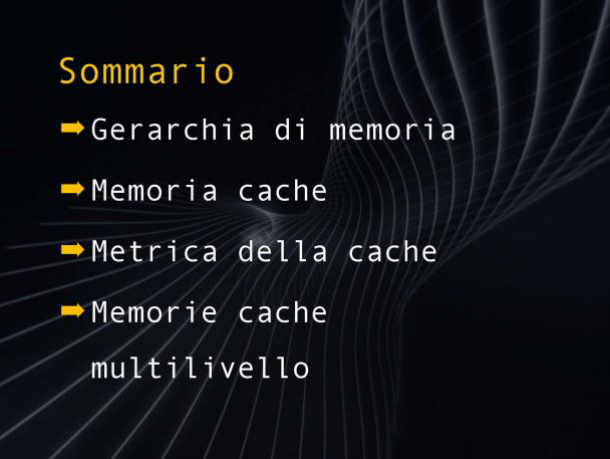
\includegraphics[width=0.40\textwidth,
                    trim=40 60 10 40, % L B R T
                    clip]
                    {images/Lez06_p01_fig_02.png}
  \caption{Sommario}
  \label{fig:Lez06_p01_fig_02}
\end{figure}
\FloatBarrier
\noindent

Iniziamo ora un ciclo di lezioni sulla gerarchia del sistema di memoria.
Il sommario è il seguente: prima introdurremo il concetto di gerarchia di memoria, poi introdurremo la memoria cache, una metrica della memoria cache e le memorie cache organizzate su più livelli o multilivello.


\section{Gerarchia di memoria}

\FloatBarrier
\begin{figure}[H]
  \centering
  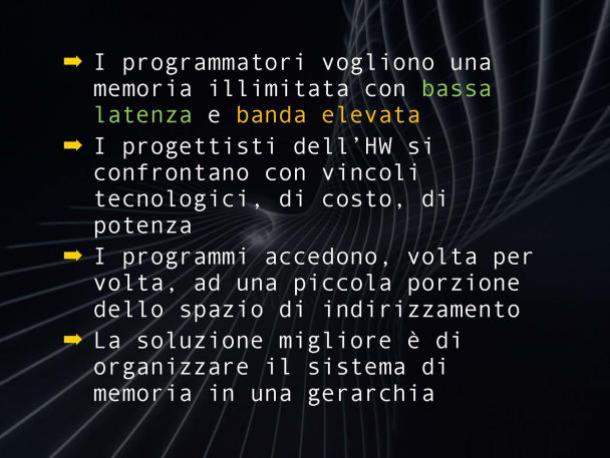
\includegraphics[width=0.40\textwidth,
                    trim=40 20 10 40, % L B R T
                    clip]
                    {images/Lez06_p01_fig_04.png}
  \caption{Gerarchia di memoria}
  \label{fig:Lez06_p01_fig_04}
\end{figure}
\FloatBarrier
\noindent

Consideriamo prima il concetto di gerarchia di memoria.
I programmatori vogliono avere una memoria illimitata con bassa latenza e banda elevata.
Dall'altra parte, i progettisti dell'hardware si confrontano con vincoli tecnologici di costo, di potenza.
L'evidenza sperimentale insegna che i programmi accedono volta per volta ad una piccola porzione dell'intero spazio di indirizzamento disponibile.
Quindi la soluzione migliore è di organizzare il sistema di memoria in una gerarchia.

\FloatBarrier
\begin{figure}[H]
  \centering
  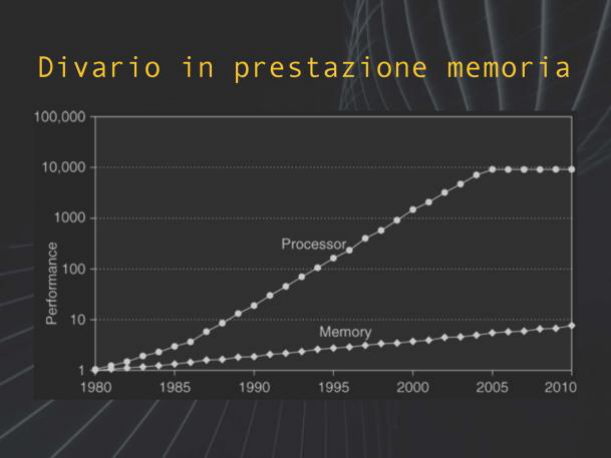
\includegraphics[width=0.60\textwidth,
                    trim=20 20 10 40, % L B R T
                    clip]
                    {images/Lez06_p01_fig_05.png}
  \caption{Gerarchia di memoria}
  \label{fig:Lez06_p01_fig_05}
\end{figure}
\FloatBarrier
\noindent

Vediamo il divario di prestazioni della memoria che si è venuto a creare negli ultimi 30-35 anni.
Vedete come sono migliorate le performance della memoria e come i processori con uno scalino attorno alla metà degli anni 80, quando sono stati introdotti i RISC e un altro ginocchio attorno al 2005, in cui lo scaling di frequenza non è stato più possibile per vincoli di potenza prevalentemente e quindi hanno preso piede i processori multicore, se questo è il miglioramento di performance per singolo core, questa curva descrive molto bene l'evoluzione.
Notate che comunque invece le prestazioni della memoria dopo i primi anni 80 sono sensibilmente più lente.
A cavallo gli anni 80 e addirittura prima spesso il processore era più lento della memoria, invece questo divario si è venuto drasticamente ad ampliare negli anni e l'aumento del numero dei core all'interno del processore, fa sì che questo numero aumenti sempre più, anche se qui sembra un platò perché è il platò per core, mentre le capacità di memoria e la banda di memoria non aumentano in maniera progressiva.

\FloatBarrier
\begin{figure}[H]
  \centering
  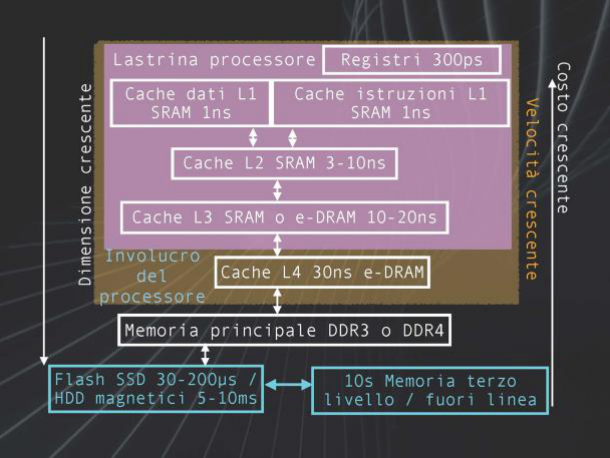
\includegraphics[width=0.70\textwidth,
                    trim=20 20 10 20, % L B R T
                    clip]
                    {images/Lez06_p01_fig_06.png}
  \caption{Gerarchia di memoria}
  \label{fig:Lez06_p01_fig_06}
\end{figure}
\FloatBarrier
\noindent

Vediamo quindi una rappresentazione grafica della gerarchia di memoria, così chiamo prima la lastrina del processore, quello che si chiama processor die in inglese.
Il primo livello, diciamo il livello più importante e veloce è quello dei registri, che sono una parte della memoria stessa, sono i registri di uso generale, l'instruction register e così via, che avete visto sicuramente nei corsi del primo livello.
Tipico tempo di accesso è 300 picosecondi, diciamo, nell'interno del periodo di clock, quindi se il clock è 3,3 GHz, il periodo è 300 picosecondi.
Ovviamente non è un numero assoluto, dipende dalla specifica implementazione, lo stessa implementazione di processore può avere varie versioni di clock a seconda di come i processori vengono bene o male durante la fase produttiva e così via.
Comunque l'ordine di grandezza è quello nell'ordine delle 300 picosecondi o un po' di più.
La cache L1 implementata con una SRAM nella parte dati ha tempi tipicamente nell'ordine di 1 nano secondo, un po' meno, un po' di più, ma quello è l'ordine di grandezza.
Analogamente la cache di istruzioni in cui raramente sono molto diverse o generalmente sono della stessa dimensione o tipicamente c'è un fattore 2 fra l'una e l'altra, ma anche questa ha la stessa velocità di accesso.
Poi le due sono collegate a una SRAM, una RAM statica di secondo livello L2 con tempi di accesso fra 3 e 10 nanosecondi, anche in questo caso dipendendo dalla dimensione del processo produttivo della SRAM.
Più è grande la SRAM, più è lungo il tempo di accesso perché più sono i livelli di codifica interni.
Notate che questa implementazione con un L1 dati e un L1 istruzione è quella che corrisponde a una architettura di Harvard modificata.

Poi in molte versioni esiste anche un L3 ancora statica, ma in qualche volta anche dinamica con tempi rispettivamente fra i 10 e i 20 nanosecondi, se siano statiche o dinamiche e soprattutto a seconda della loro dimensione.
In alcuni processori è anche possibile, all'interno del package del processore può anche esserci una cache di quarto livello L4, oramai se esiste questa di tipo e-DRAM, embedded DRAM, con tempi di accessi nell'ordine 30 nanosecondi indicativamente.

Successivamente vi è la memoria principale che, come vi ho già detto, è implementata in DDR3, double data rate 3 o double data rate 4.

Infine un livello di memorie statiche, quindi che non perdono l'informazione dopo che viene tolta l'alimentazione elettrica, tipicamente sono flash o sono dischi magnetici.

Notate i tempi di accesso di un solid state drive che è di circa 30 microsecondi nel caso sia connesso al bus PCI express e di 200 microsecondi se è connesso sul bus SATA.

Gli hard disk magnetici invece, dovendo avere parti meccaniche in traslazione e in rotazione, hanno dei tempi di accesso sulle versioni consumer più economiche, quelle che spesso si utilizzano nei normali PC di circa 10 milisecondi, corrispondente indicativamente ai dischi a 7200 giri e nei dischi di livello più professionale a 15.000 giri nell'ordine ai 5 milisecondi.

Tempo di ricerca, cioè spostamento lineare della testina più semirivoluzione del disco.
Passando dal registro fino alle memorie flash o ai dischi magnetici aumentano le dimensioni mentre viceversa i costi aumentano nella direzione opposta, cioè sia la velocità che i costi sono maggiori per i registri e L1 e sono ovviamente molto più bassi per i dischi magnetici.
Qualunque buon sistema di gerarchia di memoria deve anche prevedere una memoria di terzo livello o una memoria fuori linea, con tempi che tipicamente nella realtà delle cose sono nell'ordine della decina di secondi.

\FloatBarrier
\begin{figure}[H]
  \centering
  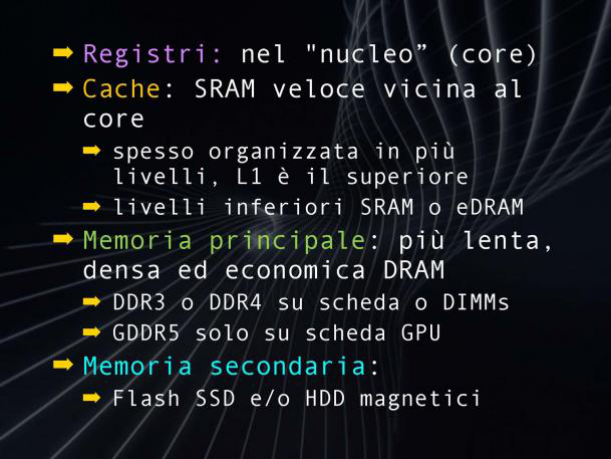
\includegraphics[width=0.60\textwidth,
                    trim=20 20 10 20, % L B R T
                    clip]
                    {images/Lez06_p02_fig_01.png}
  \caption{Gerarchia di memoria}
  \label{fig:Lez06_p02_fig_01}
\end{figure}
\FloatBarrier
\noindent

Allora, ricapitoliamo, i registri sono nel nucleo del processore o core, usiamo un nucleo giusto per farvi capire di cosa si tratta con un core, ma alla fine useremmo sempre core.
Notate che i dati vengono gestiti all'interno dei registri da parte del compilatore e dell'assemblatore.
Se tornate ai corsi al primo livello abbiamo visto diverse operazioni, ma sostanzialmente quando si fa una load in un registro, per esempio di uso generale, questa è un'operazione che è scritta di fatto nel codice assemblativo.
Quando si fa il fetch, il prelievo di un'istruzione, si va a caricare nell'instruction register, questa è un'operazione che chiaramente avviene al livello di assemblatore che scrive il codice assembler e quindi poi il codice binario.
La cache, al contrario, è una SRAM veloce, anche questa è realizzata con gli invertitori CMOS, e posta vicina al core ed è gestita dall'hardware, cioè non dal compilatore, non dall'assemblatore, ma direttamente dall'hardware.
Spesso è organizzata in più livelli e per definizione L1 è il livello superiore e l'ultimo livello tipo L3 o L4 è il livello inferiore, nel gergo comune.
I livelli inferiori sono anche essi realizzati in SRAM o, come vi ho fatto vedere nell'immagine grafica precedente, in embedded DRAM.
La memoria principale, più lenta e più densa, più economica, è realizzata con memorie dinamiche, non esistono praticamente più in commercio chip di memoria statica stand alone, cioè a sé, la SRAM è tutt'ormai integrata dentro e vicino ai processori.

Le memorie principale sono fatte in DDR3 o DDR4, che sono o saldate su scheda, nel caso di PDA o di laptop computer portati particolarmente piccole, o su dei moduli, che si chiamano Dual Inline Memory Module DIMMs, che possono essere sostituiti dall'utente.

In alcuni casi, dove, ad esempio, lo spazio è particolarmente importante, tipo in uno smartphone, la DDR3 può anche essere saldata internamente nello stesso package del chip in maniera analoga, come abbiamo visto per l'embedded DRAM precedentemente.

Questo non viene sempre fatto perché chiaramente richiede un controllo del processo da parte di chi ingegnerizza lo smartphone, in cui si limitano i livelli di flessibilità, ma chi fa volumi, può permettersi di farlo.

Nel caso di graphical processing unit, cioè le schede grafiche, si può fare anche con i GDDR5, solo saldate su scheda.
La memoria secondaria è fatta di flash e o dischi magnetici, notate che la memoria principale è gestita dal sistema operativo, così come la memoria secondaria è gestita dal sistema operativo.

Voi non scrivete come codice le specifiche istruzioni, vengono fatte delle chiamate di sistema operativo per gestire i file nella memoria, così come l'allocazione della memoria è fatta direttamente dal sistema operativo.

Su questo torneremo molto nel dettaglio nelle lezioni un po' più avanti durante il corso, ma è importante che voi capiate che i registi sono gestiti esplicitamente dall'assemblatore, quindi volendo anche dal programmatore che programmi in assembler, le cache sono gestite dall'hardware, la memoria principale e quella secondaria sono gestite dal sistema operativo.

\FloatBarrier
\begin{figure}[H]
  \centering
  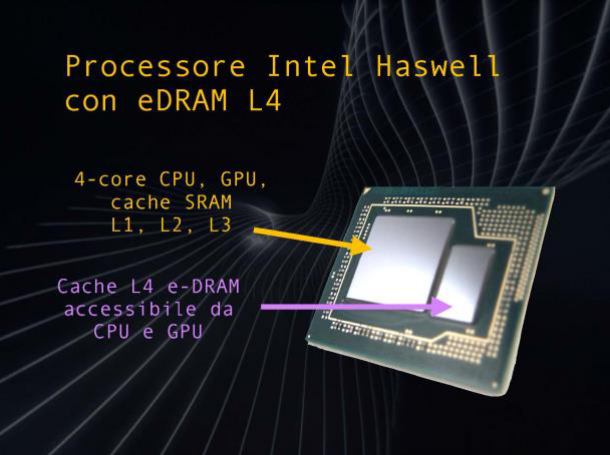
\includegraphics[width=0.60\textwidth,
                    trim=20 20 10 20, % L B R T
                    clip]
                    {images/Lez06_p02_fig_02.png}
  \caption{Gerarchia di memoria}
  \label{fig:Lez06_p02_fig_02}
\end{figure}
\FloatBarrier
\noindent

Vediamo un esempio, vi ho fatto vedere prima l'idea di un sistema multi-chip, questo è un modernissimo processore Intel, Laswell, che ha una embedded DRAM, il chip principale contiene quattro core, una CPU, contiene anche una graphical processing unit, contiene una cache SRAM di primo, poi una cache di seconda e una di terzo, e diciamo il chip più grande.
Questo stesso processo tecnologico ha 22 nanometri e anche realizzata una cache di quarto livello realizzata in embedded DRAM che è accessibile sia dalla CPU che dalla GPU.

Notate che il chip è più piccolo, ma questo permette di esempio sia tempi di accesso più bassi, velocità maggiori di accesso in termini anche di banda e soprattutto fa anche risparmiare energia perché un accesso dal, diciamo nel package costa meno energia che un accesso off package e magari verso delle DIMM.

Ricordate che caricare una capacità richiede un'energia pari a $1/2*C*V^2$, più è grande la capacità, per esempio la capacità delle piste, maggiore l'energia necessaria per caricare.

\FloatBarrier
\begin{figure}[H]
  \centering
  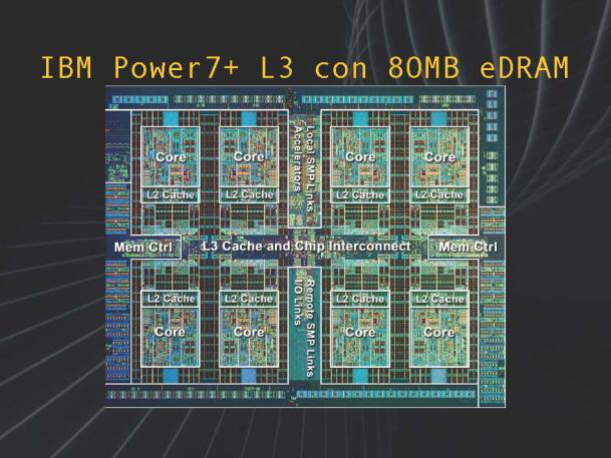
\includegraphics[width=0.60\textwidth,
                    trim=20 20 10 20, % L B R T
                    clip]
                    {images/Lez06_p02_fig_03.png}
  \caption{Gerarchia di memoria}
  \label{fig:Lez06_p02_fig_03}
\end{figure}
\FloatBarrier
\noindent

L'altro caso di un processore avanzato, l'IBM Power 7 Plus in cui vi è una L3 di ben 80 MB realizzata in embedded DRAM.
Qui vedete i core che sono abbastanza importanti ma non entremo mai nel dettaglio di questo tipo di core, con delle L1 che non si vedono chiaramente nel disegno, le L2 sono marcate, sono 512 MB, 8 core in questo caso, molti altri circuiti di cui non commentiamo e tutta queste zone attorno ai core, diciamo in modo abbastanza periodico come vedete dalle strutture, queste qui attorno sono tutte fatte di embedded DRAM per ben 80 MB.
Quindi se andate a confrontarle alle tipiche dimensioni delle L3, dei processori Intel dove nelle versioni consumer o intermedie ci sono circa 2 MB per core di L3, in questo caso abbiamo 10 MB per core e quindi 80 MB in totale.
Questo è possibile in quanto un elemento di memoria dinamico è fatto da un condensatore e un transistor, mentre un elemento statico è fatto da ben 6 transistor, quindi è possibile integrarne ben di più a parità di superficie.

\FloatBarrier
\begin{figure}[H]
  \centering
  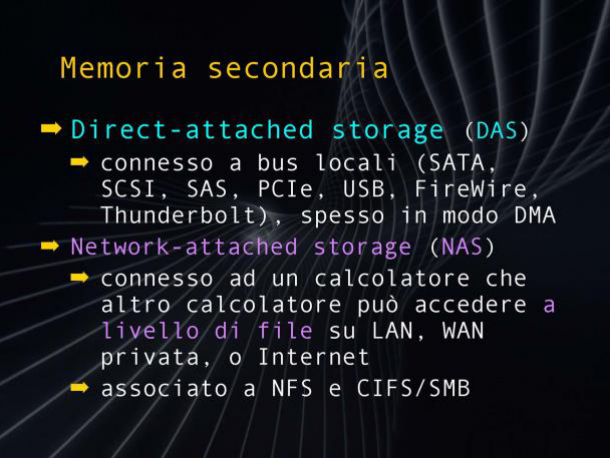
\includegraphics[width=0.60\textwidth,
                    trim=20 20 10 20, % L B R T
                    clip]
                    {images/Lez06_p02_fig_04.png}
  \caption{Gerarchia di memoria}
  \label{fig:Lez06_p02_fig_04}
\end{figure}
\FloatBarrier
\noindent

La memoria secondaria può essere connessa in diversi modi, userò gli acronimi inglesi, quello di Direct Attached Storage, quindi l'immagazzinamento connesso direttamente con l'acronimo DAS, questo è il tipico caso di qualunque computer desktop utilizzato normalmente dove il sistema di memoria secondaria è connesso a bus locali come il serialata, lo SCSI, il serial attached SCSI, lo SCSI attaccato serialmente, il PCI express, lo USB, il firewire e thunderbolt.
Tutti questi casi tranne l'USB sono connessi in DMA, quindi possono scrivere direttamente nella memoria primaria.

Esistono anche le configurazioni Network Attached Storage o NAS, dove la memoria secondaria è connessa a un calcolatore e un altro calcolatore può accedere al livello di file su una rete locale o local area network, una rete diciamo geografica, una wide area network però possibilmente privata o addirittura l'internet.

Quando voi fate un HTTP andate ad accedere un file su un computer remoto a livello di file e quello è un sistema connesso alla rete.
Questi tipi di sistemi di rete sono spesso associati a protocolli tipo il Network File Systems o NSF o Samba utilizzato da Windows.
Network File System è stato sviluppato in Italia negli anni 80 dalla SAN e questo è stato sviluppato da diversi e utilizzato abitualmente dentro nell'ambiente Windows.

\FloatBarrier
\begin{figure}[H]
  \centering
  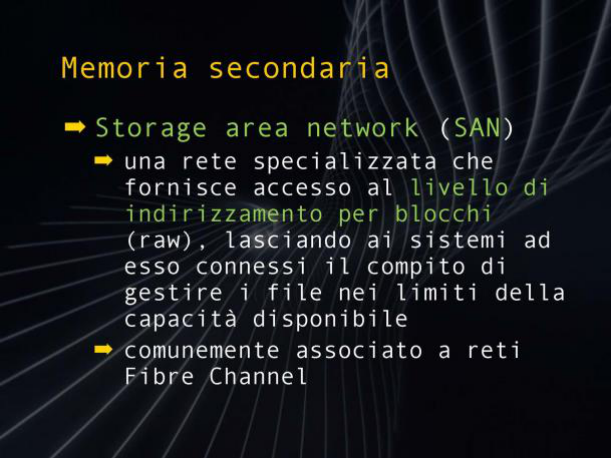
\includegraphics[width=0.60\textwidth,
                    trim=20 20 10 20, % L B R T
                    clip]
                    {images/Lez06_p02_fig_05.png}
  \caption{Gerarchia di memoria}
  \label{fig:Lez06_p02_fig_05}
\end{figure}
\FloatBarrier
\noindent

Negli ambienti professionali si usano gli Storage Area Networks o SAN in cui una rete specializzata che fornisce accesso al livello di indirizzamento per blocchi o raw data è utilizzata lasciando ai sistemi adesso connessi il compito di gestire i file nei limiti della capacità disponibile.

SAN è tipicamente associato a reti di tipo Fiber Channel.
Notate che Fiber Channel non implica necessariamente che si tratti di reti ottiche ma possono essere sia ottiche che su rame.
Queste sono reti che hanno diversi livelli di velocità partendo dal minimo di 2 GB secondo di dati raw cioè senza header, senza correzioni, senza protezioni, passando a 4, 8 e 16 GB con dei throughput netti che vanno da 99,6 MB secondo full duplex quindi per direzione fino a circa 1,6 GB full duplex.
Notate che passando dai raw data ai dati con tutti gli header con la correzione erronea chiaramente si sta perdendo quel tipico 20\% perché c'è una overhead.
E' tipicamente utilizzata per connettere, ripeto, dati, sistemi professionali di immagazzinamento di dati.

%18:01
\subsection{Memoria di terzo livello o fuori linea}

Passiamo adesso al prossimo argomento e definiamo la memoria di terzo livello o memoria fuori linea.

\FloatBarrier
\begin{figure}[H]
  \centering
  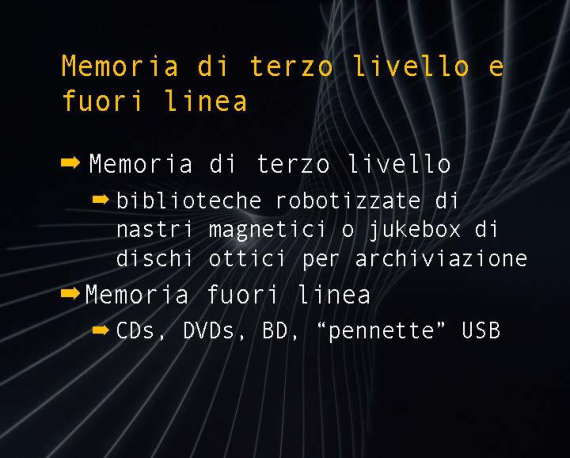
\includegraphics[width=0.60\textwidth,
                    trim=20 20 10 20, % L B R T
                    clip]
                    {images/Lez06_p02_fig_06.png}
  \caption{Gerarchia di memoria}
  \label{fig:Lez06_p02_fig_06}
\end{figure}
\FloatBarrier
\noindent

La prima è tipicamente costituita da biblioteche robotizzate di nastri magnetici o jukebox di dischi ottici per l'archiviazione.
Questo varia dagli anni agli anni, dai costi, dalla tecnologia, alla logica dei sistemi di archiviazione del terzo livello che devono costare il meno possibile per byte perché magari si vogliono mantenere diverse versioni degli stessi file archiviati per memoria storica o perché semplicemente è obbligatorio per legge; immaginate l'archiviazione di taluni dati.
Questi sono gestiti in strutture robotizzate dove ci sono dei sistemi che vanno a prendere il nastro da un archivio oppure caricano come in un jukebox musicale dischi ottici di vario tipo, Blu-ray, DVD e così via.

Si può anche avere una memoria fuori linea, quella che strutture non organizzate utilizzano, fatte da CD, DVD, Blu-ray disc o come impropriamente vengono dette pennette USB o dischi connessi su USB che vengono connessi dal singolo operatore quando serve o per archivio o per backup.

Due spunti per la riflessione: Implementare una gerarchia di memoria costa? I dati nella cache L1 sono replicati anche nelle 2, 3 o eventuale L4?

\section{Organizzazione della memoria cache}

Passiamo ora quindi a definire in modo più organizzato come funziona una memoria cache.

\FloatBarrier
\begin{figure}[H]
  \centering
  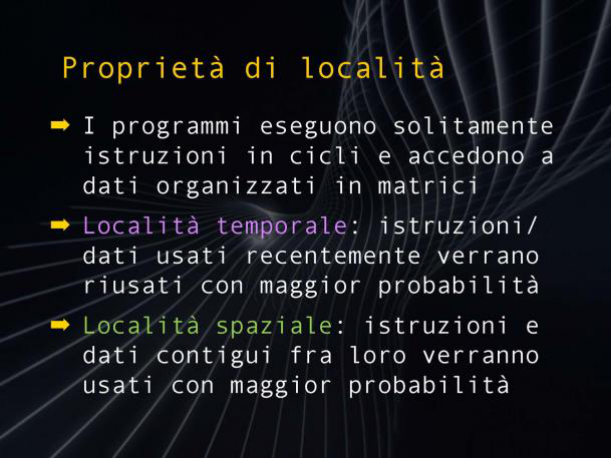
\includegraphics[width=0.60\textwidth,
                    trim=20 55 10 45, % L B R T
                    clip]
                    {images/Lez06_p03_fig_03.png}
  \caption{Organizzazione memoria cache}
  \label{fig:Lez06_p02_fig_05}
\end{figure}
\FloatBarrier
\noindent


Innanzitutto riflettiamo sulla proprietà di località.
I programmi eseguono solitamente istruzioni in cicli e accedono a dati organizzati in matrici.

Identifichiamo una località temporale dove istruzioni e dati usati recentemente verosimilmente verranno riusati con maggiore probabilità e in un tempo non molto distante da quando sono stati utilizzati per la prima volta.

Una località spaziale che ci dice che istruzioni e dati fra loro contigui nella memoria verranno usati con una maggiore probabilità.

Nel primo caso immaginate di essere all'interno di un ciclo, è molto probabile che il ciclo verrà riutilizzato più volte e quindi riaccederete agli stessi dati, in questo caso stesse istruzioni.

Nel caso degli stessi dati se per esempio fate una moltificazione riga per colonna tra due matrici, non ci sono abbastanza registri per contenere tutti gli elementi di due matrici bidimensionali, dovete tenere i dati in memoria, ma siccome la moltificazione riga per colonna verrà fatta ripetutamente, una delle righe verrà letta diverse volte, quindi è molto probabile che quei dati verranno riutilizzati.

Per quel che riguarda la località spaziale è abbastanza evidente dal semplice utilizzo di matrici, le quali, ovviamente, memorizzate sequenzialmente nella memoria principale. Ogni volta che voi fate una scansione della matrice, vi troverete verosimilmente degli indirizzi contigui.

\FloatBarrier
\begin{figure}[H]
  \centering
  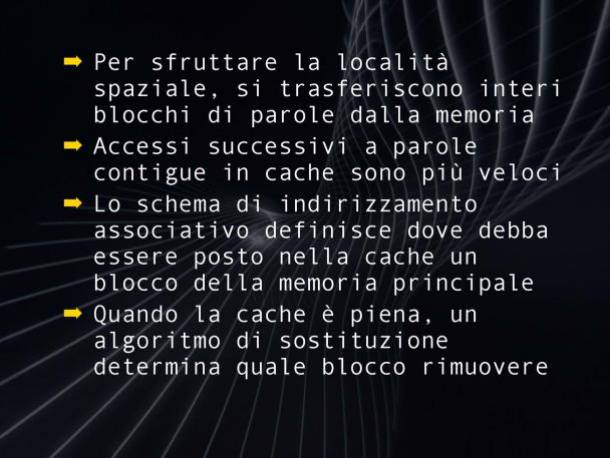
\includegraphics[width=0.60\textwidth,
                    trim=20 20 10 20, % L B R T
                    clip]
                    {images/Lez06_p03_fig_04.png}
  \caption{Gerarchia di memoria}
  \label{fig:Lez06_p03_fig_04}
\end{figure}
\FloatBarrier
\noindent


Per sfruttare la località spaziale, quindi, si trasferiscono interi blocchi di parole dalla memoria principale nella cache.
Quindi, invece di trasferire la singola parola utilizzata al sistema operativo, o anche la parola della RAM, che a volte può essere più grande perché è una linea, immaginate le parole del sistema operativo a 32 bit e la dimensione delle tipiche DIMM di 64 bit, è chiaro che quella è una parola della memoria che corrisponde alla parola del sistema operativo.

Accessi successivi a parole contigue in cache sono più veloci per i numeri che vi ho dato.
Quindi, se dobbiamo fare il prossimo accesso all'interno dello stesso blocco, accederemo la seconda volta non più con i tempi della memoria principale, ma con i tempi della cache. Quindi avremmo risparmiato notevole quantità di tempo.
Ricordate sempre l'immagine grafica che vi ho dato, gli ordini di grandezza di tempi, che, come si dice in inglese, a picture is worth a thousand words. Quell'immagine è più facile di ricordare che le parole.

Lo schema di indirizzamento associativo definisce dove debba essere posto nella cache un blocco della memoria principale. Questo è una delle parti più importanti di una cache. Come associare un blocco dalla memoria alla cache?

È anche importante sapere cosa succede quando la cache è piena. È necessario quindi un algoritmo di sostituzione che determina quale blocco rimuovere. Queste due parti fanno la differenza tra una cache ben fatta e una cache fatta meno bene.

\subsection{Cache read miss}

Chiamiamo in inglese, con il loro nome e le cose, se no in letteratura non le troverete, i cosiddetti cache read miss.

\FloatBarrier
\begin{figure}[H]
  \centering
  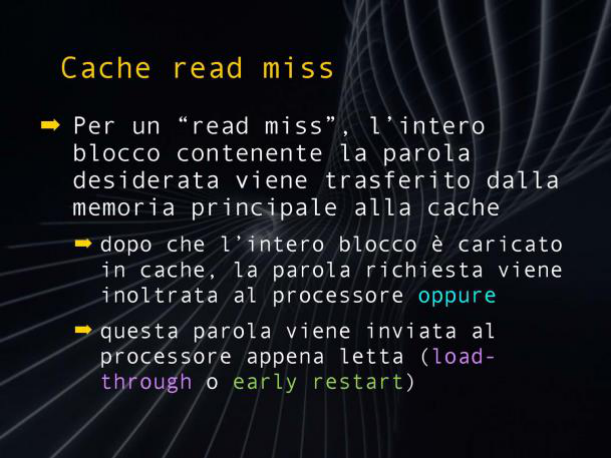
\includegraphics[width=0.60\textwidth,
                    trim=20 40 10 40, % L B R T
                    clip]
                    {images/Lez06_p03_fig_05.png}
  \caption{Gerarchia di memoria}
  \label{fig:Lez06_p03_fig_05}
\end{figure}
\FloatBarrier
\noindent


Cioè non aver pescato nella cache, siccome è brutto da dirsi in italiano mentre suona molto meglio in inglese, lo chiameremo read miss. Per un read miss, cioè quando non si è pescato nella cache, l'intero blocco contenente la parola desiderata viene trasferito dalla memoria principale alla cache.

Questo può avvenire in due modalità.

Dopo che l'intero blocco è stato caricato in cache, la parola viene richiesta dalla cache ed inoltrata al processore, questo nel caso di un read miss.

Oppure questa parola viene prima inviata al processore, per esempio caricata in un registro, se era un dato, un registro general purpose, oppure nell'instruction register, se era un'istruzione, appena questa parola viene letta. Questo in inglese si chiama load through, cioè carica attraverso o early restart, ripartenza rapida. Notate che la seconda implementazione è un po' più complicata dal punto di vista hardware, perché la parola che andiamo a pescare non necessariamente sarà la prima, potrebbe essere abbastanza in mezzo al blocco, quindi bisogna poi riorganizzare le cose. Comunque questo può consentire delle migliori performance.

%24:52

Consideriamo alcuni spunti per la riflessione, in realtà un esercizio.

Vi invito a considerare una cache dati L1 di 16 KB e una matrice bidimensionale di 1024 righe e 1024 colonne, considerate parole di 32 bit, immagazzinate in memoria per righe. Questa è una cosa abbastanza semplice.
Vi invito ora a scrivere due versioni di un codice costituito sostanzialmente da due soli cicli for annidati, non importa cosa avvenga all'interno del ciclo annidato, immaginate anche qualcosa di banale, con uno solo dei due cicli che sfrutti la cache. Potete capire con quale ciclo riuscite a usare la cache e quale non usarlo.

Notate che questa normalmente è un'operazione trasparente al programmatore, ma in realtà è buona cosa che il programmatore sia consapevole, ad esempio, della dimensione della cache o che comunque il compilatore lo sia, in modo tale da poter eventualmente rimodificare il loop per rendere il codice più efficiente, valorizzando le dimensioni della cache.

\subsection{Metrica della cache}
Passiamo ora al prossimo argomento e vi do ora rapidamente alcuni elementi di metrica della cache.

\FloatBarrier
\begin{figure}[H]
  \centering
  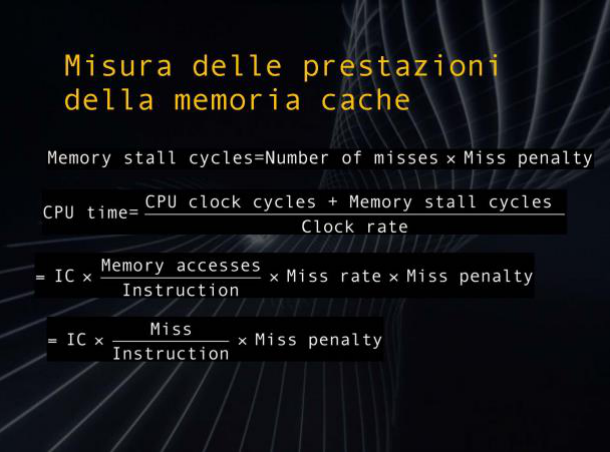
\includegraphics[width=0.60\textwidth,
                    trim=20 20 10 20, % L B R T
                    clip]
                    {images/Lez06_p04_fig_02.png}
  \caption{Gerarchia di memoria}
  \label{fig:Lez06_p04_fig_02}
\end{figure}
\FloatBarrier
\noindent

Consideriamo come misura delle prestazioni della memoria cache alcune grandezze.
I cosiddetti memory stall cycle, cioè i cicli di stallo della memoria, sono pari al numero dei miss per la penalità del miss.
Quello che conta è il tempo complessivo di processore, il CPU time, e questo è dato dal numero di cicli di clock utilizzati dal processore più il numero di cicli di clock in cui la memoria è in stallo.
Ovviamente in tempo assoluto va diviso per il clock rate, o in alternativa, moltiplicato per il periodo del clock, che è la stessa cosa.

Questa esplicitandola è pari all'instruction count, cioè al numero delle istruzioni, moltiplicata per il numero di accessi alla memoria per istruzione, moltiplicata per il tasso di miss, cioè il miss rate, moltiplicato per la penalità del miss.

Riesplicitandola si può anche scrivere in una forma pratica, cioè come instruction count per miss diviso instruction, cioè quante miss ci sono per istruzione per miss penalty, generalmente questo è un numero minore di uno, però casi molto particolari in cui non c'è né la istruzione load né il dato in cache, può anche comportare che quell'istruzione abbia in linea di principio un miss per instruction di 2, ma è un caso un po' particolare, non ci vogliamo soffermare su questo.

E consideriamo un esempio numerico dell'uso di una cache.

\FloatBarrier
\begin{figure}[H]
  \centering
  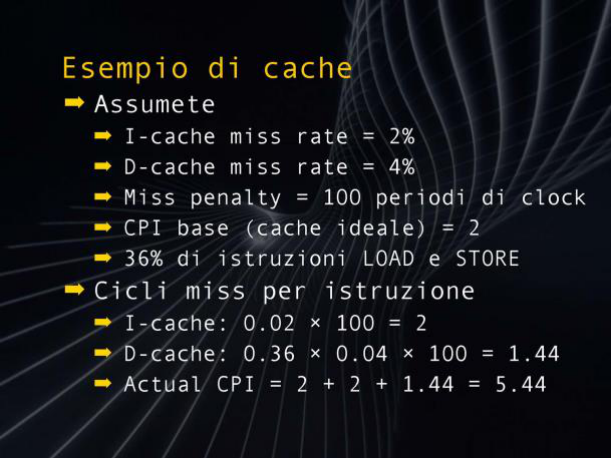
\includegraphics[width=0.50\textwidth,
                    trim=20 40 10 40, % L B R T
                    clip]
                    {images/Lez06_p04_fig_03.png}
  \caption{Gerarchia di memoria}
  \label{fig:Lez06_p04_fig_03}
\end{figure}
\FloatBarrier
\noindent

Assumete che la cache istruzione abbia un miss rate del 2\%, la cache dati abbia un miss rate del 4\%, una miss penalty di 100 periodi di clock e un clock per instruction base, cioè per una cache ideale pari a 2, cioè ci sono due istruzioni, cioè due clock per ogni istruzione, diciamo questa è un'ipotesi.
E assumiamo anche che il 36\% di istruzioni siano load e store, non facciamo una differenza tra i tempi di esecuzione di una load e di una store né del tempo di accesso in questo momento.

I cicli miss per istruzione che ci vengono fuori sono per la cache istruzione pare al 2\% moltiplicato i centri periodi di clock necessari e ci vengono due cicli per una miss nell'istruzione.

Per i dati abbiamo il tasso di istruzioni load e store che è il 36\%, moltiplicato il tasso di miss nel cache dati che è il 4\% per cento, che è il numero dei periodi di clock necessario per accedere a memoria e si arriva a 1,44.

Quindi il cosiddetto actual clock per instruction, cioè il numero di colpi di clock per istruzione reale è pari a 2, quello originario, più 2 per le istruzioni, più 1,4 per i dati, pari a 5,44. Quindi il numero originario è peggiorato in maniera ben sensibile.

Consideriamo anche un'altra grandezza, il cosiddetto average memory access time, perché il tempo per colpire, cioè per raggiungere la memoria, è importante per la valutazione delle prestazioni.

\FloatBarrier
\begin{figure}[H]
  \centering
  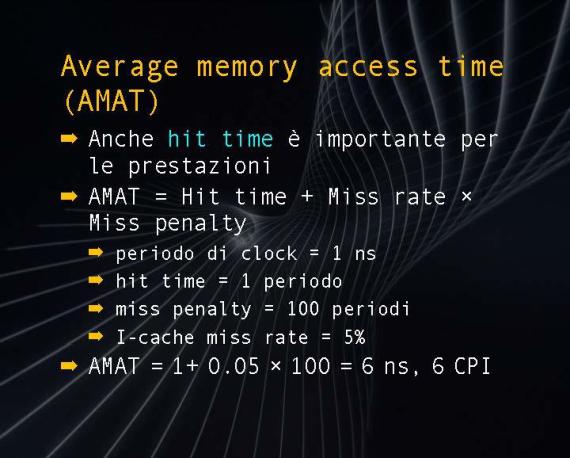
\includegraphics[width=0.50\textwidth,
                    trim=20 40 10 40, % L B R T
                    clip]
                    {images/Lez06_p04_fig_04.png}
  \caption{Gerarchia di memoria}
  \label{fig:Lez06_p04_fig_04}
\end{figure}
\FloatBarrier
\noindent

Il cosiddetto AMAT è dato dal tempo per raggiungere le istruzioni più il tasso di miss moltiplicato per la penalità di miss.
Facciamo un esempio, per un periodo di clock di 1 nanosecondo è un hit time pari a 1 periodo e una miss penalty di 100 periodi di clock e un'ipotesi di instruction cache miss rate del 5\%, troviamo un AMAT, un tempo di accesso media alla memoria, pari a 1 che era il valore tipico del hit time, più 5\% per 100 e arriviamo a 6 nanosecondi, cioè invece che i 5 che avremmo avuto solo con la cache penalty e più l'1 del hit time.

Nel caso la penalità sia inferiore e il hit time rimanga uguale, facciamo un esempio di una miss penalty di 20 periodi, quindi se la miss penalty fosse di 20 periodi il nostro tempo passerebbe da 1 a 2, quindi la variazione sarebbe ancora più importante.

Vedremo nel proseguo delle lezioni che fra hit time e cache penalty e miss rate in realtà ci sono dei trade off, cioè dei compromessi da prendere.
Avere un basso hit time spesso è al costo di avere un grande miss rate e viceversa.

\subsection{Memorie cache multilivello}

Passiamo ora al prossimo argomento, le memorie cache multilivello.

\FloatBarrier
\begin{figure}[H]
  \centering
  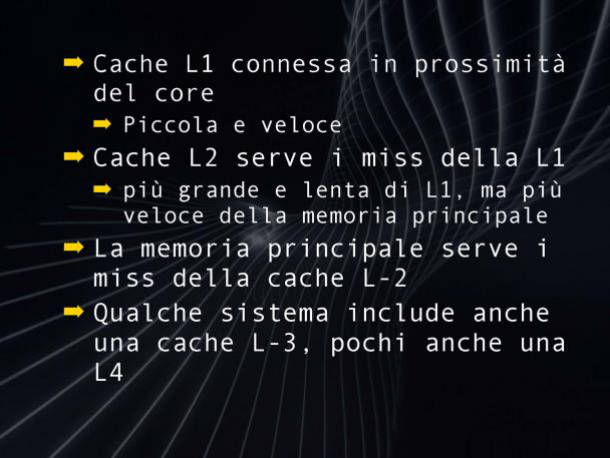
\includegraphics[width=0.50\textwidth,
                    trim=20 20 10 20, % L B R T
                    clip]
                    {images/Lez06_p04_fig_06.png}
  \caption{Gerarchia di memoria}
  \label{fig:Lez06_p02_fig_05}
\end{figure}
\FloatBarrier
\noindent

Consideriamo che le cache L1 sono connesse in prossimità del core per ridurre i percorsi, sono piccole e veloci, la cache L2 serve i miss della L1, questo è l'obiettivo primario di avere una L2, è più grande e più lenta della L1 ma più veloce comunque della memoria principale.
La memoria principale serve i miss della L2 e come vi ho detto qualche sistema include anche una cache L3 che serve i miss della L2, pochi sistemi ancora per il momento hanno anche una L4 che serve i miss della L3.

\FloatBarrier
\begin{figure}[H]
  \centering
  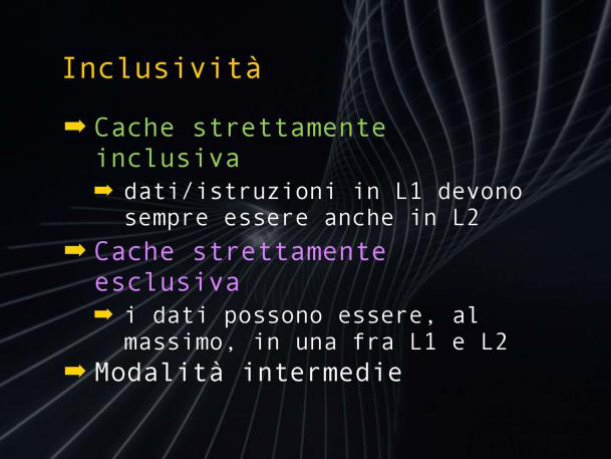
\includegraphics[width=0.50\textwidth,
                    trim=20 20 10 20, % L B R T
                    clip]
                    {images/Lez06_p05_fig_01.png}
  \caption{Gerarchia di memoria}
  \label{fig:Lez06_p05_fig_01}
\end{figure}
\FloatBarrier
\noindent

Consideriamo il concetto di inclusività per ricollegarci alla domanda fattavi precedentemente.
Definiamo una cache strettamente inclusiva, una cache in cui i dati o le istruzioni nelle L1 devono sempre essere anche in L2, al contrario una cache strettamente esclusiva è tale per cui i dati possono essere al massimo in una fra L1 e L2, ovviamente possono non essere in nessuna delle cache nel caso in cui le dati sono nella memoria principale e nel caso di assenza di L3 o L4, ma la differenza di fondo è che ogni dato in L1 è sicuramente stato copiato in L2 nelle memorie strettamente inclusive.

Esistono anche delle modalità intermedie utilizzate tempo addietro da Intel, adesso non tanto comuni ma possibili, in cui la memoria è inclusiva ma non obbligatoriamente.

Consideriamo in realtà soltanto questi due casi estremi.

\FloatBarrier
\begin{figure}[H]
  \centering
  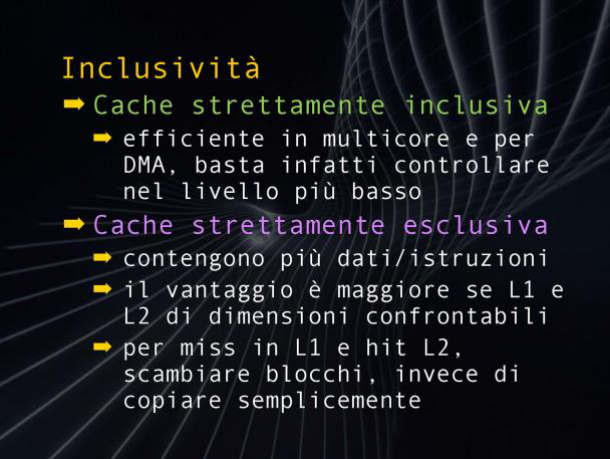
\includegraphics[width=0.50\textwidth,
                    trim=20 20 10 20, % L B R T
                    clip]
                    {images/Lez06_p05_fig_02}
  \caption{Gerarchia di memoria}
  \label{fig:Lez06_p05_fig_02}
\end{figure}
\FloatBarrier
\noindent

Nel caso di una cache strettamente inclusiva, ci accorgiamo subito che questa è particolarmente efficiente per architetture multicore e per l'accesso diretto alla memoria, il DMA, perché basta infatti controllare nel livello più basso della memoria, quindi se ad esempio abbiamo un L1 e L2, se il dato è in L2 allora è sicuramente anche in L1.
Per le cache strettamente esclusive, queste hanno il vantaggio che a parità di transistor complessivi contengono più dati e più istruzioni.
Questo vantaggio è particolarmente notevole se L1 e L2 hanno dimensioni confrontabili, ad esempio in alcuni produttori la somma delle due L1, cioè la somma delle dimensioni delle due L1 è pari alla dimensione della L2 che è condivisa.
Per un miss in L1 e un hit in L2 è necessario scambiare i blocchi nelle memorie strettamente esclusive e invece di semplicemente copiare i dati dall'L2 e dall'L1.
Questo richiede il doppio delle operazioni e richiede ovviamente un insieme di circuteria che permetta di trasferire un blocco dall'L1 indietro verso la L2.
Questo ovviamente complica e soprattutto dissipa un po' più di energia che nel caso dell'L1, come vedete diciamo ci sono pro e contro nelle due implementazioni.

\FloatBarrier
\begin{figure}[H]
  \centering
  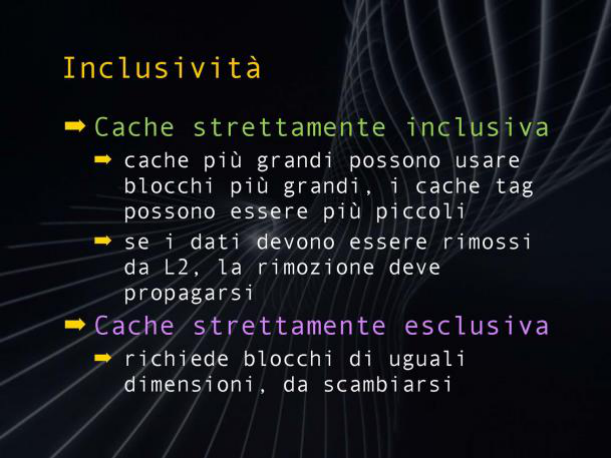
\includegraphics[width=0.50\textwidth,
                    trim=20 20 10 20, % L B R T
                    clip]
                    {images/Lez06_p05_fig_03}
  \caption{Gerarchia di memoria}
  \label{fig:Lez06_p05_fig_03}
\end{figure}
\FloatBarrier
\noindent

Sempre sulla memoria strettamente inclusiva, se si hanno delle cache di livello più basso, tipo L2 e L3, più grandi, allora lì si possono anche usare blocchi più grandi. In questo modo si risparmiano cache tag che vedremo fra poco nei bit di tag.

Se i dati devono essere rimossi dalla L2, la rimozione deve propagarsi anche alla L1, quindi diciamo che bisogna fare nel  caso delle strettamente inclusive più lavoro, in qualche modo duale al lavoro doppio che si faceva per lo scambio nella L1 e L2 delle strettamente esclusive.
Per le strettamente esclusive invece è necessario che i blocchi siano di dimensioni uguali nelle L1 e L2 in modo da poter essere scambiati, quindi ci sono dei pro e dei contro in entrambe le soluzioni.

\FloatBarrier
\begin{figure}[H]
  \centering
  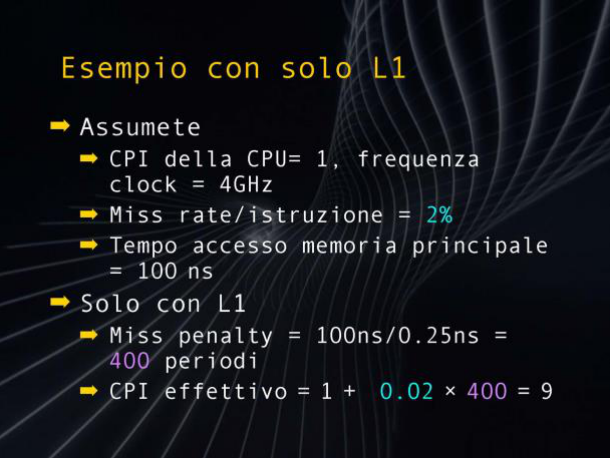
\includegraphics[width=0.50\textwidth,
                    trim=20 20 10 20, % L B R T
                    clip]
                    {images/Lez06_p05_fig_04}
  \caption{Gerarchia di memoria}
  \label{fig:Lez06_p05_fig_04}
\end{figure}
\FloatBarrier
\noindent

Esempio con soltanto L1.
Assumete i seguenti dati.
Un clock per instruction della CPU pari a 1, una frequenza di clock di 4 GHz, un miss rate per istruzione del 2\%, un tempo di accesso alla memoria principale di 100 ns.
Solo con la L1 troviamo che la penalità per un miss è pari a 100 ns diviso 0,25 ns che è il periodo, pari a 400 periodi.
Il clock per instruction effettivo, cioè il numero di cicli di clock effettivo per istruzione diventa quindi 1, che era quello nativo, più 0,02 per 400 ben 9.
Quindi abbiamo peggiorato le performance del nostro processore a causa dei miss da 1 a 9.

\FloatBarrier
\begin{figure}[H]
  \centering
  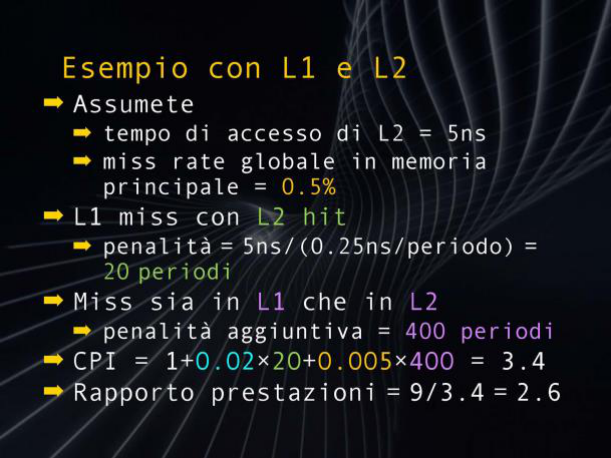
\includegraphics[width=0.50\textwidth,
                    trim=20 20 10 20, % L B R T
                    clip]
                    {images/Lez06_p05_fig_05}
  \caption{Gerarchia di memoria}
  \label{fig:Lez06_p05_fig_05}
\end{figure}
\FloatBarrier
\noindent

Se però nell'esempio introduciamo sia una L1 che una L2 con le stesse performance dell'L1, ma in cui assumiamo che il tempo di accesso all'L2 sia di 5 ns, che il miss rate globale in memoria principale sia del 0,5\%, quindi del più basso di quello dell'L1, perché la L2 è più grande, l'L1 miss con un L2 hit, cioè non è in L1 ma è in L2 il dato, sia una penalità di 5 ns diviso 0,25 ns per periodo pari a 20 periodi.

Nel caso in cui invece vi sia un miss sia in L1 che in L2, diciamo il caso più sfortunato, abbiamo una penalità aggiuntiva di 400 periodi per accedere alla memoria principale e quindi il clock per instruction, cioè il numero di clock per istruzione effettivo è dato da 1, più quello derivante dal miss in L1 e hit in L2, più i 400 cicli con la probabilità però dello 0,5\% che ci dà 3.4.
Notate che in questo caso la penalità dell'L1 si somma a quella dell'L2, perché prima abbiamo visto in L1, ci voleva un certo tempo e solo dopo che abbiamo visto che non era in L1 siamo andati a vedere in L2.
Il rapporto delle prestazioni però comunque migliora rispetto al caso di assenza di L2 con il rapporto 9 che era il clock per instruction del caso della sola L1 su 3,4 che il valore appena trovato, quindi c'è un miglioramento avendo la L2 con queste caratteristiche di un fattore ben 2,6.

\FloatBarrier
\begin{figure}[H]
  \centering
  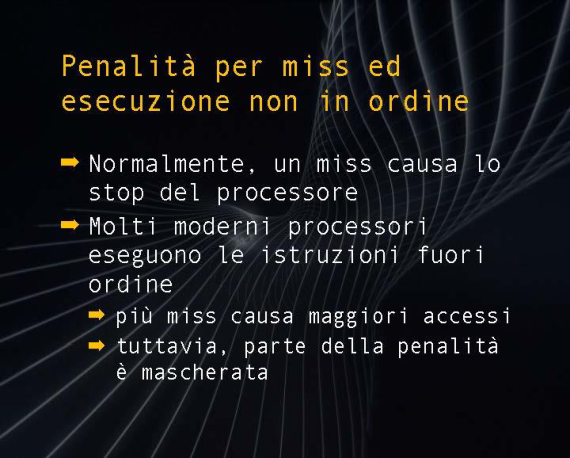
\includegraphics[width=0.50\textwidth,
                    trim=20 20 10 20, % L B R T
                    clip]
                    {images/Lez06_p05_fig_06}
  \caption{Gerarchia di memoria}
  \label{fig:Lez06_p05_fig_06}
\end{figure}
\FloatBarrier
\noindent

Ora vi do anche un ultimo punto di riflessione, la penalità per miss e l'esecuzione non in ordine.
Noi normalmente assumiamo in questa lezione che un miss causa lo stop del processore, cioè il processore non può fare null'altro. Però molti moderni processori eseguono le istruzioni fuori dall'ordine in cui sono scritte.
Di questo vi è stato detto brevemente nel corso del primo livello ci saranno una serie di lezioni proprio su queste cose più avanti nel corso di questo corso.
Quindi è vero che l'esecuzione fuori ordine porta da un aumento dei miss, cioè che ci sono più miss causa il maggior numero di accessi perché alcune istruzioni vengono già messe nella pipeline eseguite ma non vengono come dire committed in inglese, cioè non vengono completate fino alla fine. Però tuttavia parte della penalità del miss è mascherata dall'esecuzione fuori ordine.

Perché?

Perché riusciamo comunque a fare qualche parte di istruzioni utili mentre stiamo attendendo che i dati arrivino da una cache di livello più basso dalla memoria principale.


Concludiamo questa lezione con degli spunti per la riflessione e degli interrogativi a cui risponderemo nelle lezioni successive.
Dove può essere piazzato un blocco nel livello più alto, per esempio nell'L1? Come si fa a sapere se un blocco è nel livello più alto? Quale blocco deve essere sostituito in caso di miss? E infine cosa succede in scrittura?